\setchapterimage[6cm]{chapter/country/Political_Map_of_the_World_2013.png}
%\setchapterstyle{kao}
\setchapterpreamble[u]{\margintoc}
\chapter{Analysis of aspects of modern countries\protect\footnotemark}
\labch{country}

\footnotetext{\href{https://en.wikipedia.org/wiki/World_map}{Political map of the world}. 
	Author: \href{https://commons.wikimedia.org/wiki/File:Political_Map_of_the_World,_2013.png}{Central Intelligence Agency / 2015 /  Creative Commons Attribution License}.}

The chapter is devoted to the study of countries based on the knowledge base of the Wikidata international project. SPARQL queries were used in order to analyse and compare "countries" objects in Wikidata. A list of all currently existing countries, a list of countries ordered by date of creation, a list of demonyms of countries were generated. A bubble chart with the forms of government of countries and a graph of neighboring countries were constructed. In addition, conclusions were drawn regarding the completeness of the Wikidata for this topic.

%%%%%%%%%%%%%%%%%%%%%%%%%%%%%%%%%%%%%%%%%%%%%%%%%%%%%%%
\section{Instances}

Let's build a list of all countries in English and Russian.

\begin{lstlisting}[ language=SPARQL, 
caption={\href{https://w.wiki/k6L}{List of countries in English and Russian}},
label=lst:country]
SELECT ?country ?label_en ?label_ru
WHERE
{
	?country wdt:P31 wd:Q6256. # country
	?country rdfs:label ?label_en filter (lang(?label_en) = "en").
	?country rdfs:label ?label_ru filter (lang(?label_ru) = "ru").
}
\end{lstlisting}

SPARQL query (listing ~\ref{lst:country}), 205 results (2017), 175 results (2020).

Examples of the most complete and well-developed countries on the Wikidata include \wdqName{United States of America}{30}, \wdqName{Canada}{16}, \wdqName{Spain}{29}.

Almost empty and uninformative countries include \wdqName{Sahrawi Arab Democratic Republic}{40362}, \wdqName{Transnistria}{907112}, \wdqName{Kosovo}{1246}.


%%%%%%%%%%%%%%%%%%%%%%%%%%%%%%%%%%%%%%%%%%%%%%%%%%%%%%%
\section{Age of countries}

Let's build a list of countries sorted by the date of the country's foundation (the first mention of the country).

\begin{lstlisting}[ language=SPARQL, 
caption={\href{https://w.wiki/k6M}{List of `instances of` "countries sorted by inception" }},
label=lst:age_of_country, 					
]
SELECT ?country ?countryLabel ?inception
WHERE
{
	?country wdt:P31 wd:Q6256. # country
	?country wdt:P571 ?inception. # inception
	
	SERVICE wikibase:label { bd:serviceParam wikibase:language "en" }
}

ORDER BY (?inception)
}
\end{lstlisting}

SPARQL query (listing ~\ref{lst:age_of_country}), 112 results (2017), 199 results (2020).

As a result of the query, a list of countries with the dates of their creation was received. For example: \wdqName{Russia}{159} - Jan 1 0862, \wdqName{Kosovo}{1246} - Feb 17 2008, \wdqName{South Sudan}{958} - Jul 9 2011.

According to ProWD \wdqName{France}{142} and \wdqName{Israel}{801} are the leaders in the number of objects (127 objects) among all countries. \wdqName{Land of Nod}{1929769} and \wdqName{Polska Ludowa}{11165755} have the least number of objects (3 objects).


\subsection{Completeness of Wikidata}

Let's analyze the completeness of the Wikidata.

According to the "Russian classification of countries of the world" there are 251 countries on earth.

This task does not take into account ancient, non-existent states (for example: \wdqName{Assyria}{41137}), since they are not a "country" object but a "former country" object. Let us note that the number of former countries is an order of magnitude greater than the existing countries.

According to the category of \href{https://w.wiki/dWv}{"Alphabetical list of countries and territories"} in Russian Wikipedia, there are 252 countries.

According to the category of \href{https://en.wikipedia.org/wiki/List_of_sovereign_states}{"List of sovereign states"} in English Wikipedia, there are 206 countries.

It is not always possible to specify the exact date of the country's foundation for various reasons: absence, lack or inconsistency of written sources. For example, the basis of the Old Russian state is associated with the vocation of Varangian prince Rurik in 862, but there is no exact date (object \wdqName{Russia}{159}). Also, some modern countries were preceded by a number of others and the date of formation of which of them should be considered as the date of creation of the country is an open question (for example, \wdqName{Mongolia}{711}).

\subsection{Countries with an unfilled inception}

Let's display a list of countries with an empty "inception of" property.

\begin{lstlisting}[ language=SPARQL, 
caption={\href{https://w.wiki/k6q}{List of `instances of` "countries without a inception" }},
label=lst:without_inception
]
SELECT ?country ?countryLabel 
WHERE
{
	?country wdt:P31 wd:Q6256. # country
	
	MINUS { ?country wdt:P571 [] } . # inception of country is empty
	SERVICE wikibase:label { bd:serviceParam wikibase:language "en" }
}
\end{lstlisting}

SPARQL query (listing ~\ref{lst:without_inception}), 100 results (2017), 7 results (2020).

So, on March 6 2017, the Wikidata contains 100 out of 198 entries about the currently existing countries with an unknown year of the country's foundation.

%%%%%%%%%%%%%%%%%%%%%%%%%%%%%%%%%%%%%%%%%%%%%%%%%%%%%%%
\section{List of demonyms in English}

Let's build a list of countries that have demonyms in English.

\begin{lstlisting}[ language=SPARQL, 
caption={\href{https://w.wiki/mro}{List of countries with demonyms in English}},
label=lst:demonym, 
]
SELECT ?country ?countryLabel 
WHERE
{
	?country wdt:P31 wd:Q6256.       #country
	?country wdt:P1549 ?demonym .    #demonym
	
	FILTER((LANG(?demonym)) = "en")
	SERVICE wikibase:label { bd:serviceParam wikibase:language "en" }
}

GROUP BY ?country ?countryLabel
\end{lstlisting}

SPARQL query (listing ~\ref{lst:demonym}), 197 results (2017), 162 results (2020).

As of April 26 2017, the Wikidata contains 197 of the 202 countries with demonyms.

\subsection{List of demonyms}

Let's build a list of all demonyms in English.

\begin{lstlisting}[ language=SPARQL, 
caption={\href{https://w.wiki/mrp}{List of demonyms in English}},
label=lst:list_demonym, 
]
SELECT ?country ?countryLabel ?demonym
WHERE
{
	?country wdt:P31 wd:Q6256.      #country
	?country wdt:P1549 ?demonym .   #demonym
	
	FILTER((LANG(?demonym)) = "en")
	SERVICE wikibase:label { bd:serviceParam wikibase:language "en" }
}
\end{lstlisting}

SPARQL query (listing ~\ref{lst:list_demonym}), 237 results (2017), 213 results (2020).

On April 27 2017, the Wikidata contains 237 filled demonyms.

\subsection{Countries with unfilled demonyms}

Let's build a list of countries which do not have demonyms in English.

\begin{lstlisting}[ language=SPARQL, 
caption={\href{https://w.wiki/myi}{List of countries without demonyms in English}},
label=lst:without_demonym, 
]
SELECT ?country ?countryLabel 
WHERE
{
	?country wdt:P31 wd:Q6256.              # country
	MINUS { ?country wdt:P1549 ?demonym.    # except with demonyms
		FILTER((LANG(?demonym)) = "en") # in English
	}    
	
	SERVICE wikibase:label { bd:serviceParam wikibase:language "en" }
}
GROUP BY ?country ?countryLabel
\end{lstlisting}

SPARQL query (listing ~\ref{lst:without_demonym}), 5 results (2017), 20 results (2020).

On April 27 2017, the Wikidata comprise 5 of the 202 countries with unfilled demonyms.

\subsection{Number of completed demonyms in countries}

Let`s display the list of countries, ordered by the number of demonyms filled in Wikidata.

\begin{lstlisting}[ language=SPARQL, 
caption={\href{https://w.wiki/mrq}{Count of demonyms in countries}},
label=lst:count_demonym, 
]
SELECT  ?country ?countryLabel (count(*) as ?count)
WHERE
{
	?country wdt:P31 wd:Q6256.      #country
	?country wdt:P1549 ?demonym .   #demonym
	SERVICE wikibase:label { bd:serviceParam wikibase:language "en" }
}

GROUP BY ?country ?countryLabel 
ORDER BY DESC(?count)
\end{lstlisting}

SPARQL query (listing ~\ref{lst:count_demonym}),199 results (2017), 167 results (2020).

The United States of America object contains the maximum number of demonyms - 41, Great Britain - 40, Germany -40, Canada - 36 and Russia - 34.

%%%%%%%%%%%%%%%%%%%%%%%%%%%%%%%%%%%%%%%%%%%%%%%%%%%%%%%
\section{Basic forms of government}

Let`s construct a bubble diagram of the forms of government of countries.

\begin{lstlisting}[ language=SPARQL, 
caption={\href{https://w.wiki/mrr}{Basic form of government ranking}},
label=lst:form_of_government
]
SELECT ?bfog ?form (count(*) as ?count)
WHERE 
{
	?country wdt:P31 wd:Q6256.
	?country wdt:P122 ?bfog .
	
	OPTIONAL {
		?bfog rdfs:label ?form
		filter (lang(?form) = "ru")
	}
}
GROUP BY ?bfog ?form
ORDER BY DESC(?count) ASC(?form)
\end{lstlisting}

SPARQL query (listing ~\ref{lst:form_of_government}),199 results (2017), 30 results (2017), 29 results (2020).

As a result of the query, we get a bubble chart with the most popular forms of government in countries.

\begin{figure}
	{
		\setlength{\fboxsep}{0pt}%
		\setlength{\fboxrule}{1pt}%
		\fcolorbox{gray}{gray}{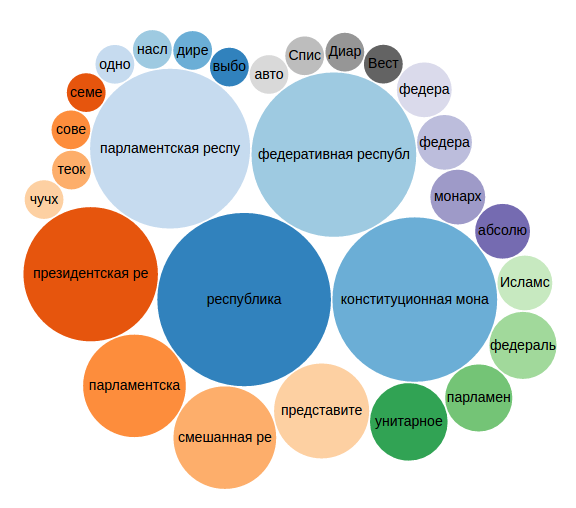
\includegraphics[width=\linewidth]{./chapter/country/Bubble_chart_forms_of_government_countries_according_to_Wikidata.png}}%
	}
	\caption{Bubble chart forms of government countries, 2017
	\\ The popular forms of government of the countries are the republic (in 20 countries), the constitutional monarchy (in 18 countries), the federal republic (in 18 countries), the parliamentary republic (in 17 countries) and the presidential system (in 11 countries) for 2017.
}%
	\label{fig:bubble_chart_forms_of_government_countries_2017}%
\end{figure}

\begin{figure}
	{
		\setlength{\fboxsep}{0pt}%
		\setlength{\fboxrule}{1pt}%
		\fcolorbox{gray}{gray}{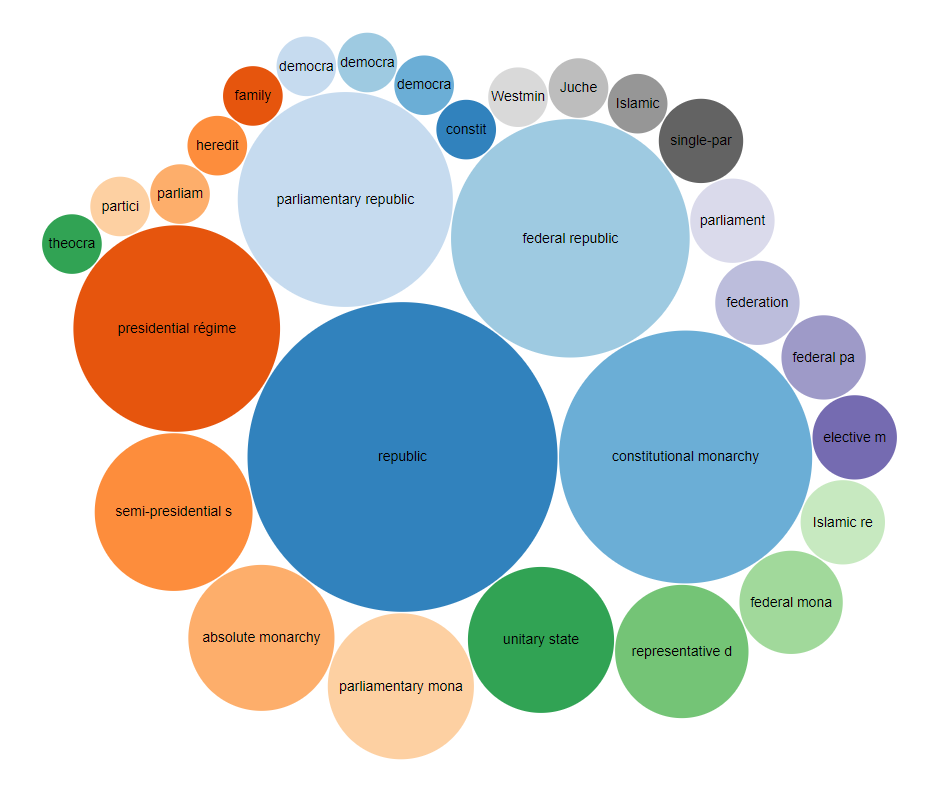
\includegraphics[width=\linewidth]{./chapter/country/Bubble_chart_forms_of_government_countries_according_to_Wikidata_2020.PNG}}%
	}
	\caption{Bubble chart forms of government countries, 2020
	\\ 
	The popular forms of government of the countries are the republic (in 27 countries), the constitutional monarchy (in 18 countries), the federal republic (in 16 countries), the parliamentary republic (in 13 countries) and the presidential system (in 12 countries) for 2020.
}%
	\label{fig:bubble_chart_forms_of_government_countries_2020}%
\end{figure}

%%%%%%%%%%%%%%%%%%%%%%%%%%%%%%%%%%%%%%%%%%%%%%%%%%%%%%%
\section{Neighboring countries}

We will construct a graph of neighboring countries.

\begin{lstlisting}[ language=SPARQL, 
caption={\href{https://w.wiki/mrs}{Neighboring countries graph}},
label=lst:neighboring_countries
]
SELECT ?country ?countryLabel ?sharesBorderWith ?sharesBorderWithLabel
WHERE
{
	?country wdt:P31 wd:Q6256.
	
	SERVICE wikibase:label { bd:serviceParam wikibase:language "en" }
	OPTIONAL { ?country wdt:P47 ?sharesBorderWith . }
}
\end{lstlisting}

SPARQL query (listing ~\ref{lst:neighboring_countries}), 795 results (2017), 698 results (2020).

\begin{figure}
	{
		\setlength{\fboxsep}{0pt}%
		\setlength{\fboxrule}{1pt}%
		\fcolorbox{gray}{gray}{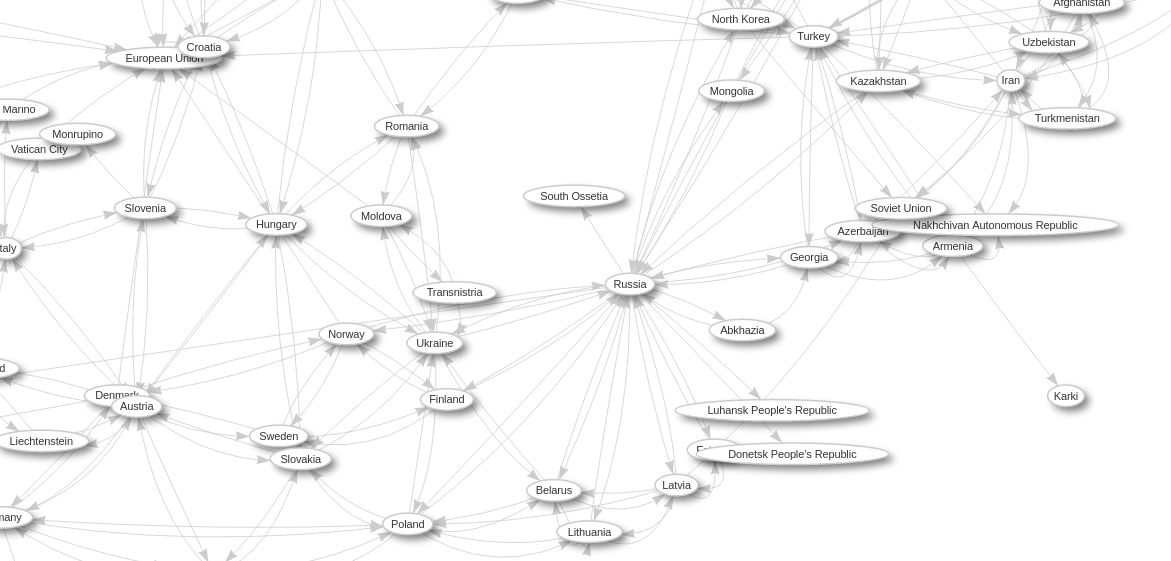
\includegraphics[width=\linewidth]{./chapter/country/Neighboring_countries_graph_according_to_Wikidata.png}}%
	}
	\caption{Neighboring countries graph, 2017.
	}%
	\label{fig:neighboring_countries_2017}%
\end{figure}

\begin{figure}
	{
		\setlength{\fboxsep}{0pt}%
		\setlength{\fboxrule}{1pt}%
		\fcolorbox{gray}{gray}{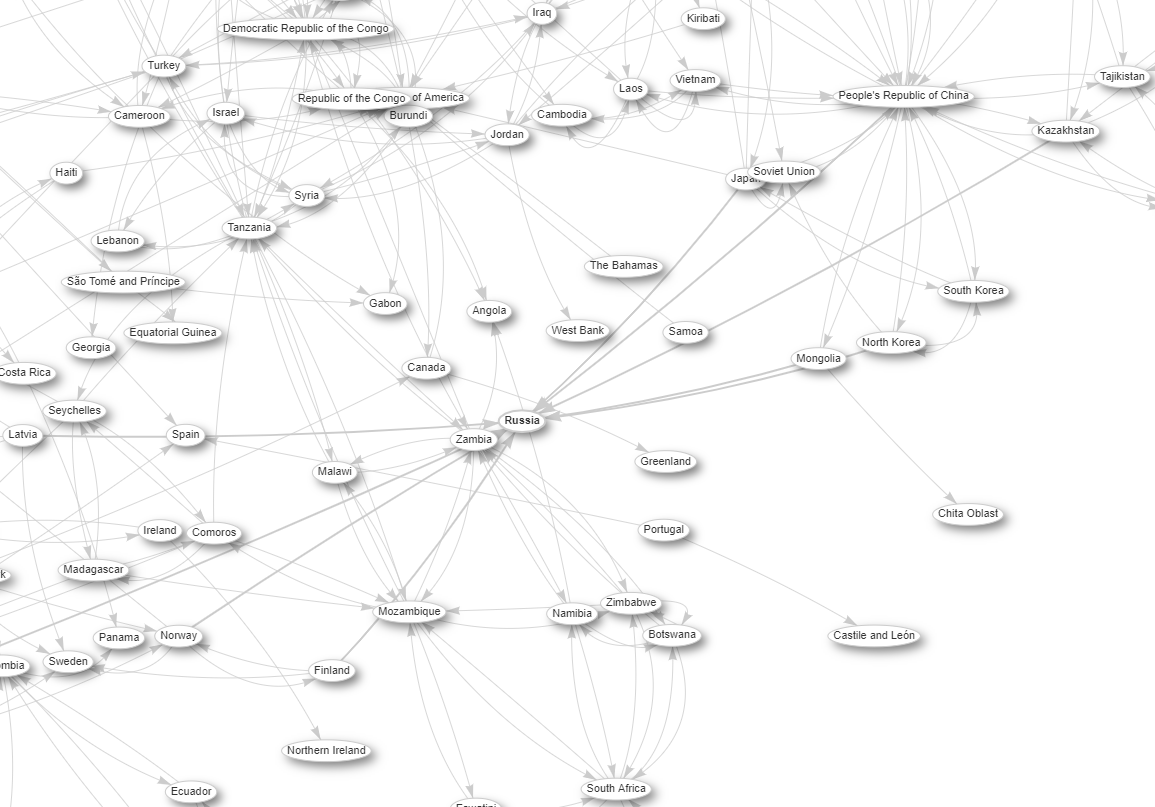
\includegraphics[width=\linewidth]{./chapter/country/Neighboring_countries_graph_in_russian_according_to_Wikidata_2020_en_upload.png}}%
	}
	\caption{Neighboring countries graph, 2020.
	}%
	\label{fig:neighboring_countries_2020}%
\end{figure}

As a result of the query, we get a graph with 787 edges on 2017 (fig. ~\ref{fig:neighboring_countries_2017}) and 698 edges on 2020 (fig. ~\ref{fig:neighboring_countries_2020}), where the edge is a neighborhood between the two countries. The graph represents several connected components, since there are island countries that do not have neighbors (for example, Mauritius, Maldives, Madagascar).

%%%%%%%%%%%%%%%%%%%%%%%%%%%%%%%%%%%%%%%%%%%%%%%%%%%%%%%
\section{Tasks}
\begin{enumerate}
	\item For each country display its flag and motto.
	\item Draw a map with the marked capitals of all the existing countries.
	\item Calculate the first five countries with the largest population density for each continent.
	\item Construct a column diagram showing the distribution of the number of countries by form of government. Estimate whether this distribution is a heavy tail.
	\item Build list the countries ordered by the number of neighbors. Which countries have the maximum and minimum number of neighbors, what is the average number of neighbors? Is there a correlation between this index and some other parameter of the countries?
\end{enumerate}
